\documentclass[]{article}
\usepackage{graphicx}
\usepackage[table]{xcolor}
\usepackage{natbib}



%plots path
\graphicspath{ {plots/} }


\title{Impacts of sagebrush vegetation in a desert climate on the atmospheric boundary layer}
\author{Byron Eng, Matthew Moody, and Travis Morrison}

\begin{document}

\maketitle

%\begin{abstract}
%XXX
%\end{abstract}

\section{Introduction}
The Mountain Terrain Atmospheric Modeling and Observations (MATERHORN, \citealt{MATERHORN}) Program provides an array of atmospheric observations suitable to investigate and advance many areas of scientific interest. Near-surface flow in areas with vegetation and complex terrain remains an area of weakness in current Numerical Weather Prediction (NWP) models, turbulence closure models, and boundary layer parameterizations \citep{MATERHORN}. In this study, boundary layer characteristics from two MATERHORN observation sites (Sagebrush and Playa) are investigated. The contrast in surface roughness between the two sites are expected to affect dissipation, mixing, and heat flux.

\section{Results}
%background on data 
Data was provided from the Sagebrush and Playa sites for October 18-19th. Both sites harvested data from meteorological towers equipped with fast response sonic anemometers (C-SAT), and finewire thermocouples at multiple heights (18.8 m, 10.15 m, 5.87 m, 2.04 m, and 0.55 m for Sagebrush and 25.5 m,19.4 m, 10.4 m, 5.3 m, 2.02 m, 0.61m for Playa). The variables measured were the three components of velocity (captured at 20 Hz), temperature, relative humidity (captured at 1 Hz). As a post-processing step the velocity data components were rotated to a Cartesian coordinate system based on 30-minute block averages, with $u$ denoting the mean wind direction, $v$ as the velocity horizontally perpendicular to the mean flow, and $w$ as the vertical velocity. Fluctuations from the mean were also calculated from a 30-minute block average. 

% Byron talks about part 1)
$\bar{u}$, $\bar{v}$, and $\bar{w}$ were calculated using the rotated velocity data. $\bar{v}$ and $\bar{w}$ are close to zero (order of $10^{-4}$ and $10^{-5}$, respectively) for the entire observation period (Figures~\ref{fig:playarotate} and~\ref{fig:sagerotate}) verifying that the rotation algorithm performed as expected. Velocity perturbations ($u'$, $v'$, and $w'$) were calculated using these mean values. Temperature perturbations ($T'$) and 30-minute block averages ($\bar{T}$) were also calculated.

Sensible heat flux ($H_s$) was calculated for both sites using Equation~\ref{eq:hs}. Where $C_p$ is the specific heat of dry air at constant pressure, and $\rho$ is the density of air.

\begin{equation}
H_s = C_p \cdot \rho \cdot \overline{w'T'}
\label{eq:hs}
\end{equation}

Turbulence kinetic energy ($TKE$) was calculated for both sites using Equation~\ref{eq:tke}. 

\begin{equation}
TKE = \frac{1}{2}~ \overline{u'^2 + v'^2 + w'^2}
\label{eq:tke}
\end{equation}

Figure~\ref{fig:hstke} shows comparisons for $H_s$ and $TKE$ at both sites. Vegetation at the Sagebrush site appears to inhibit sensible heat flux at heights below 2 m, indicating surface heat storage induced by vegetation. Sagebrush near-surface $TKE$ also appears inhibited by vegetation which is compensated by a sharp $TKE$ increase just above the surface. The Playa site shows a more uniform distribution of $TKE$ and $H_s$ at all observed heights.

\begin{equation}
L = \frac{u_*}{\kappa~ \overline{w'T'}}
\label{eq:L}
\end{equation}

Equation~\ref{eq:L} shows the calculation used for Obukhov length ($L$), where $\kappa$ is the Kolmogorov constant (assumed equal to 0.4), and $u_* = \sqrt[4]{\overline{u'w'}^2 + \overline{v'w'}^2}$. The time series of $L$ (Figure~\ref{fig:L}) show that the Playa had more near-surface instability during the observation period. However, approximately 2 meters above the surface $L$ at the Playa remained near zero for the majority of the observation period while $L$ fluctuated between positive and negative with greater amplitude at the Sagebrush site. 

\begin{figure}
	\centering
	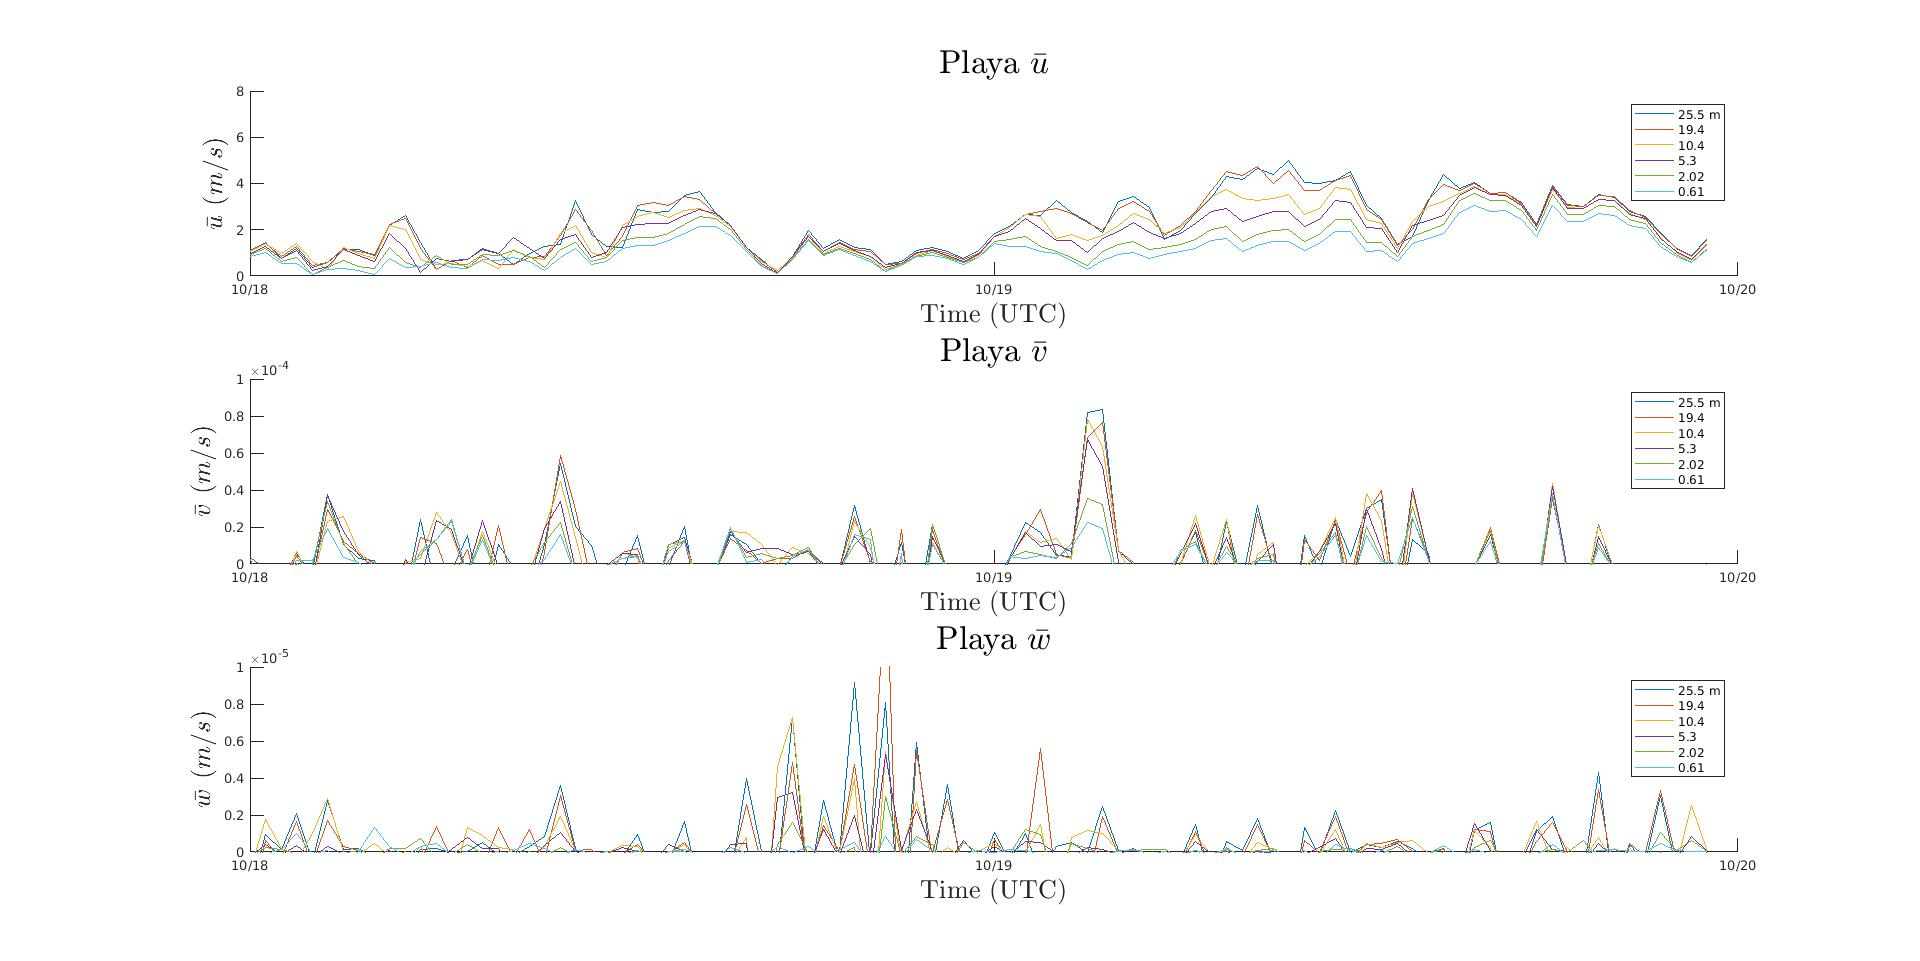
\includegraphics[width=\textwidth]{playarotate}
	\caption{30-minute block averages of $\bar{u}$, $\bar{v}$, and $\bar{w}$ from the Playa.}
	\label{fig:playarotate}
\end{figure}

\begin{figure}
	\centering
	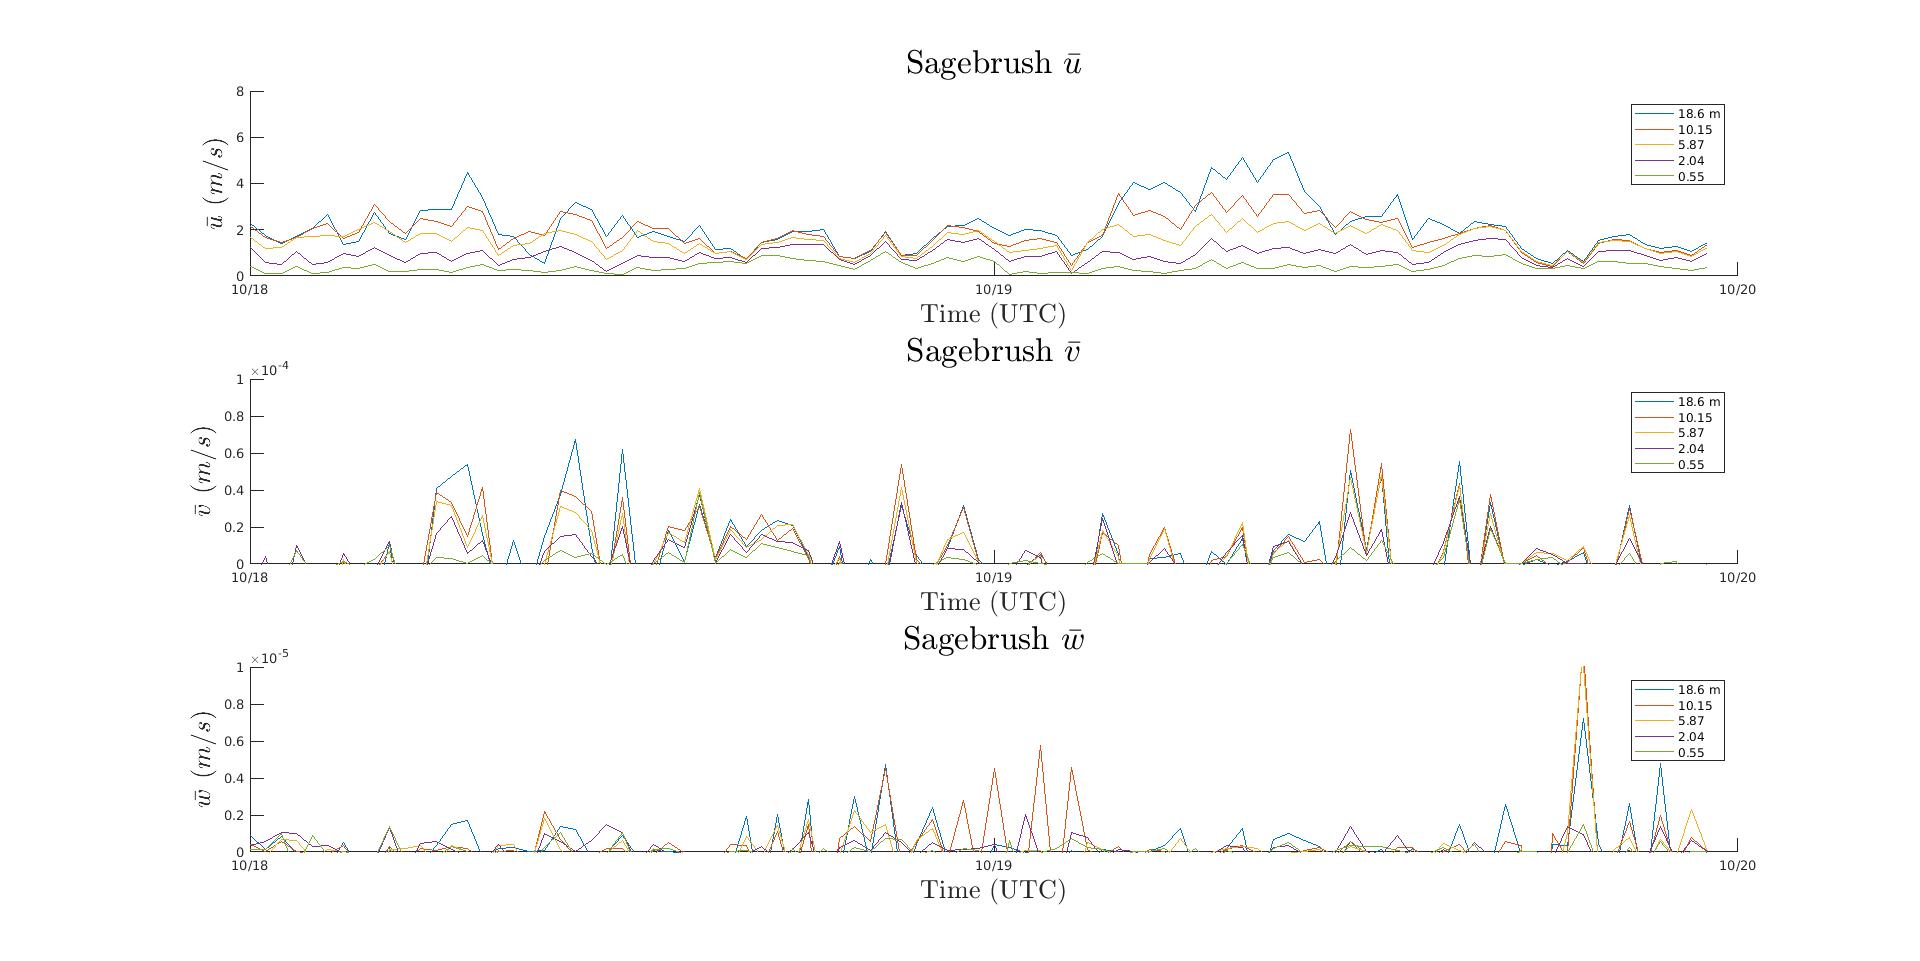
\includegraphics[width=\textwidth]{sagerotate}
	\caption{30-minute block averages of $\bar{u}$, $\bar{v}$, and $\bar{w}$ from the Sagebrush site.}
	\label{fig:sagerotate}
\end{figure}

%I don't think these fit in anywhere, but if we can find a way to use them that would be cool!
%\begin{figure}
%	\centering
%	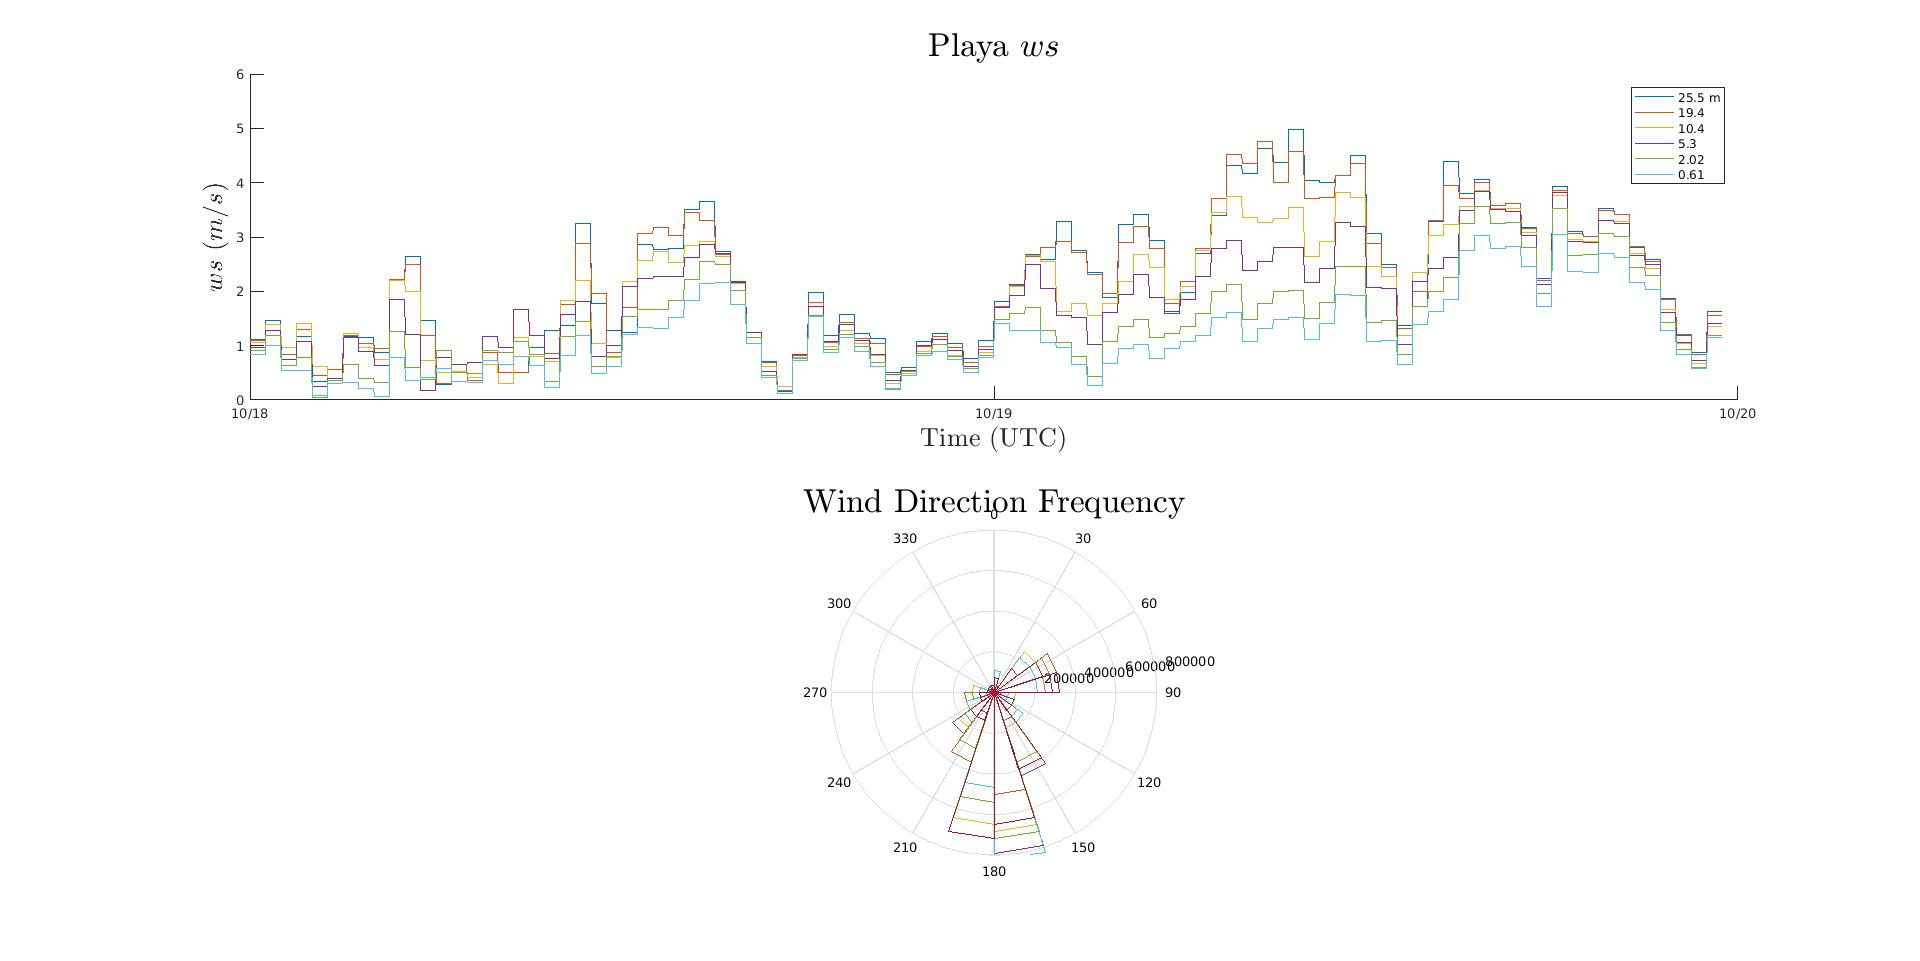
\includegraphics[width=\textwidth]{playawind}
%	\caption{Wind speed and wind rose for the Playa. Wind rose wedge size shows the frequency of datapoints from each direction.}
%	\label{fig:playawind}
%\end{figure}
%
%\begin{figure}
%	\centering
%	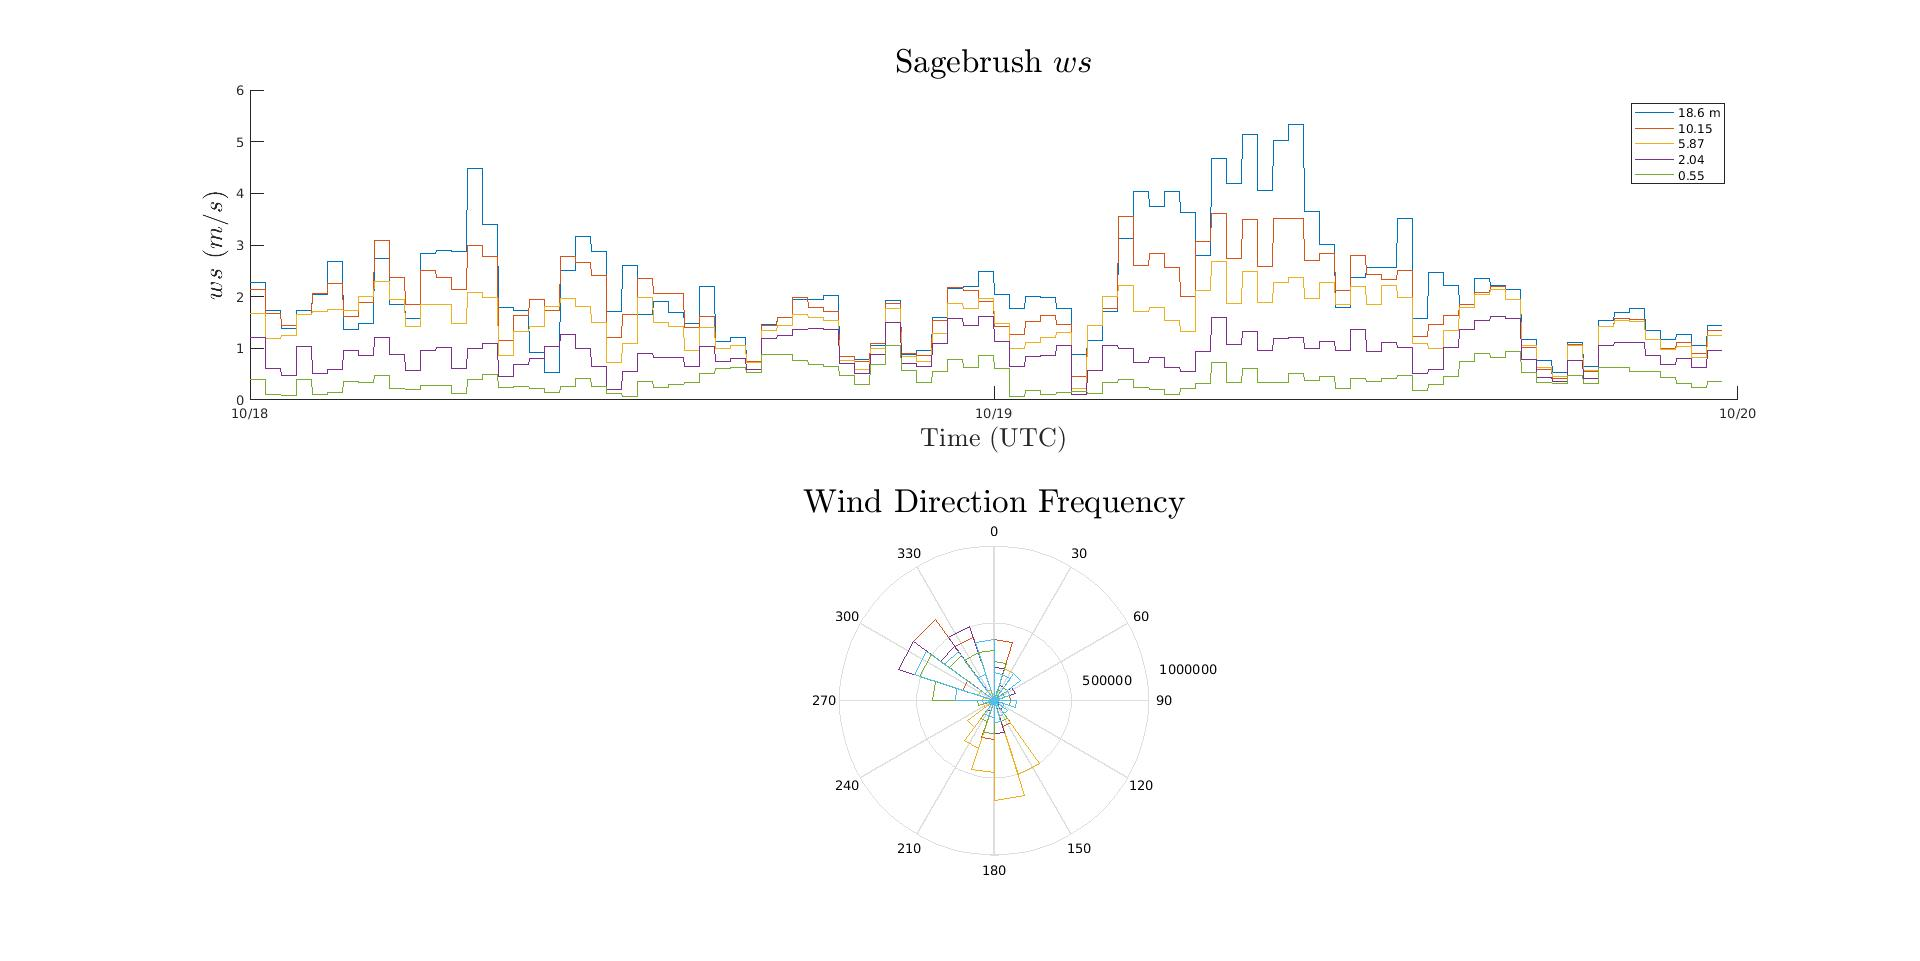
\includegraphics[width=\textwidth]{sagewind}
%	\caption{Wind speed and wind rose for the Sagebrush site. Wind rose wedge size shows the frequency of datapoints from each direction.}
%	\label{fig:sagewind}
%\end{figure}

\begin{figure}
	\centering
	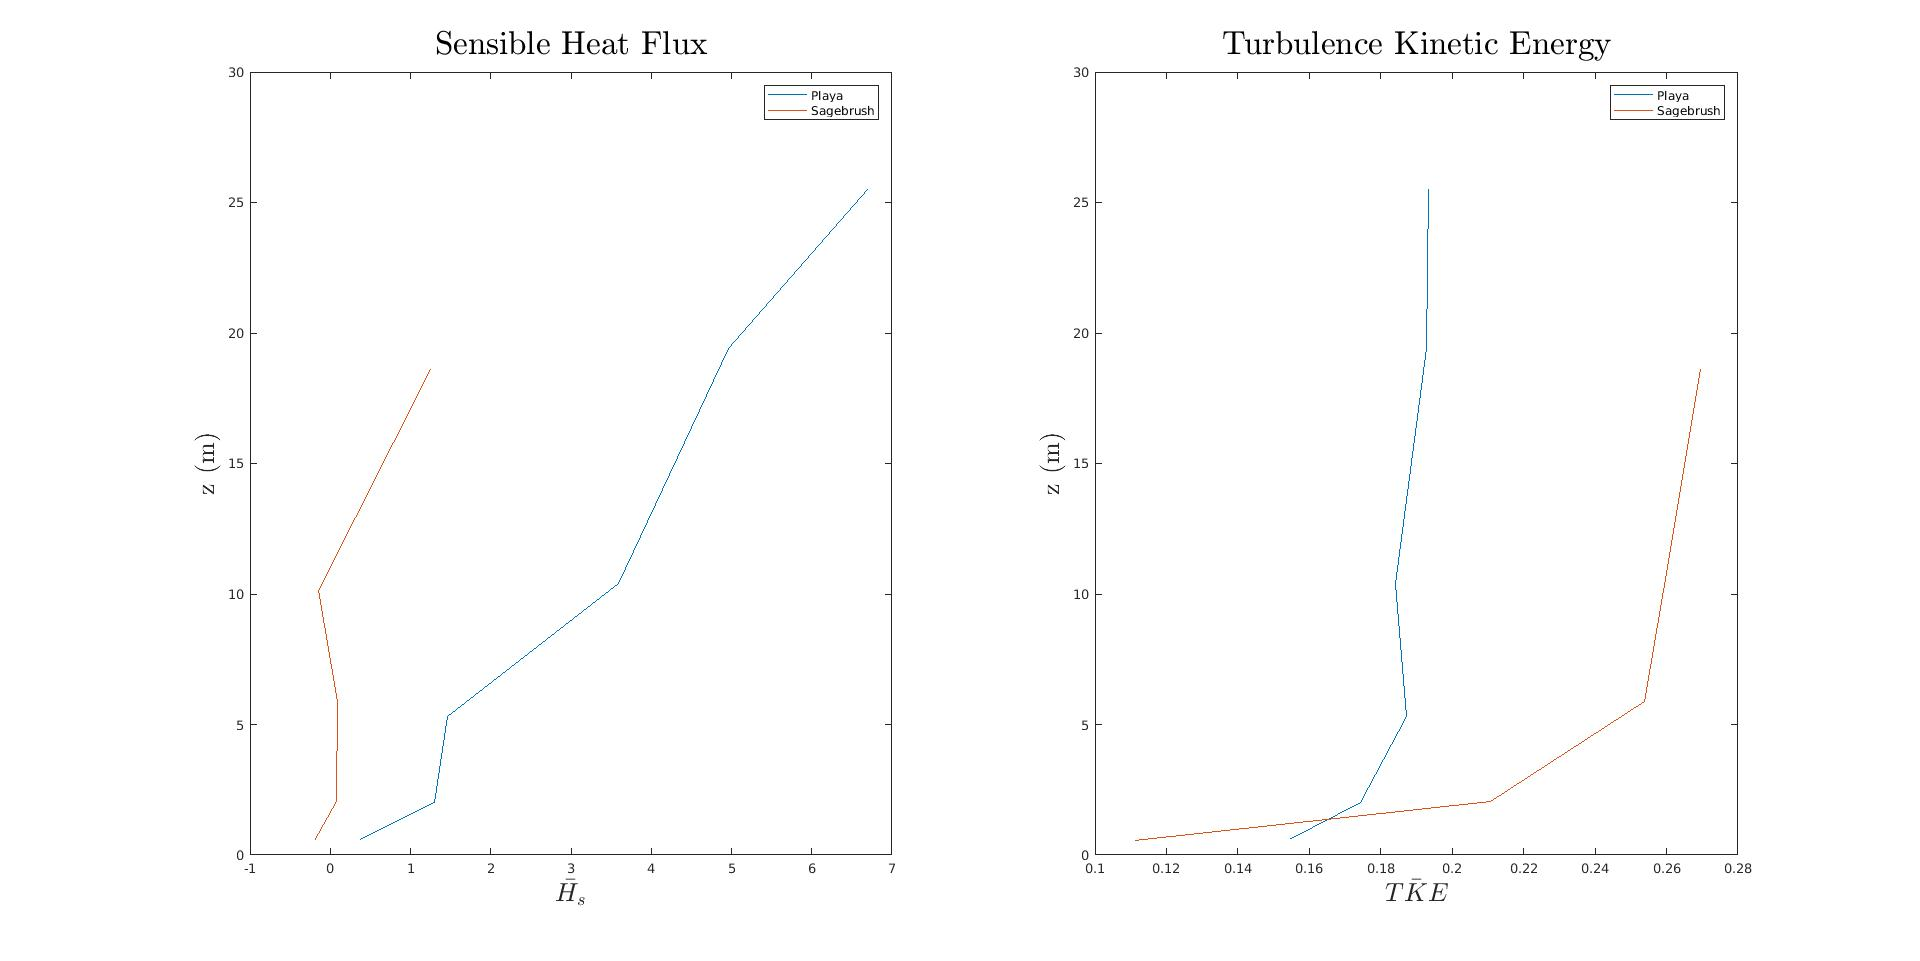
\includegraphics[width=\textwidth]{hstke}
	\caption{$H_s$ and $TKE$ comparisons. Values at each height were averaged over the observation period.}
	\label{fig:hstke}
\end{figure}

\begin{figure}
	\centering
	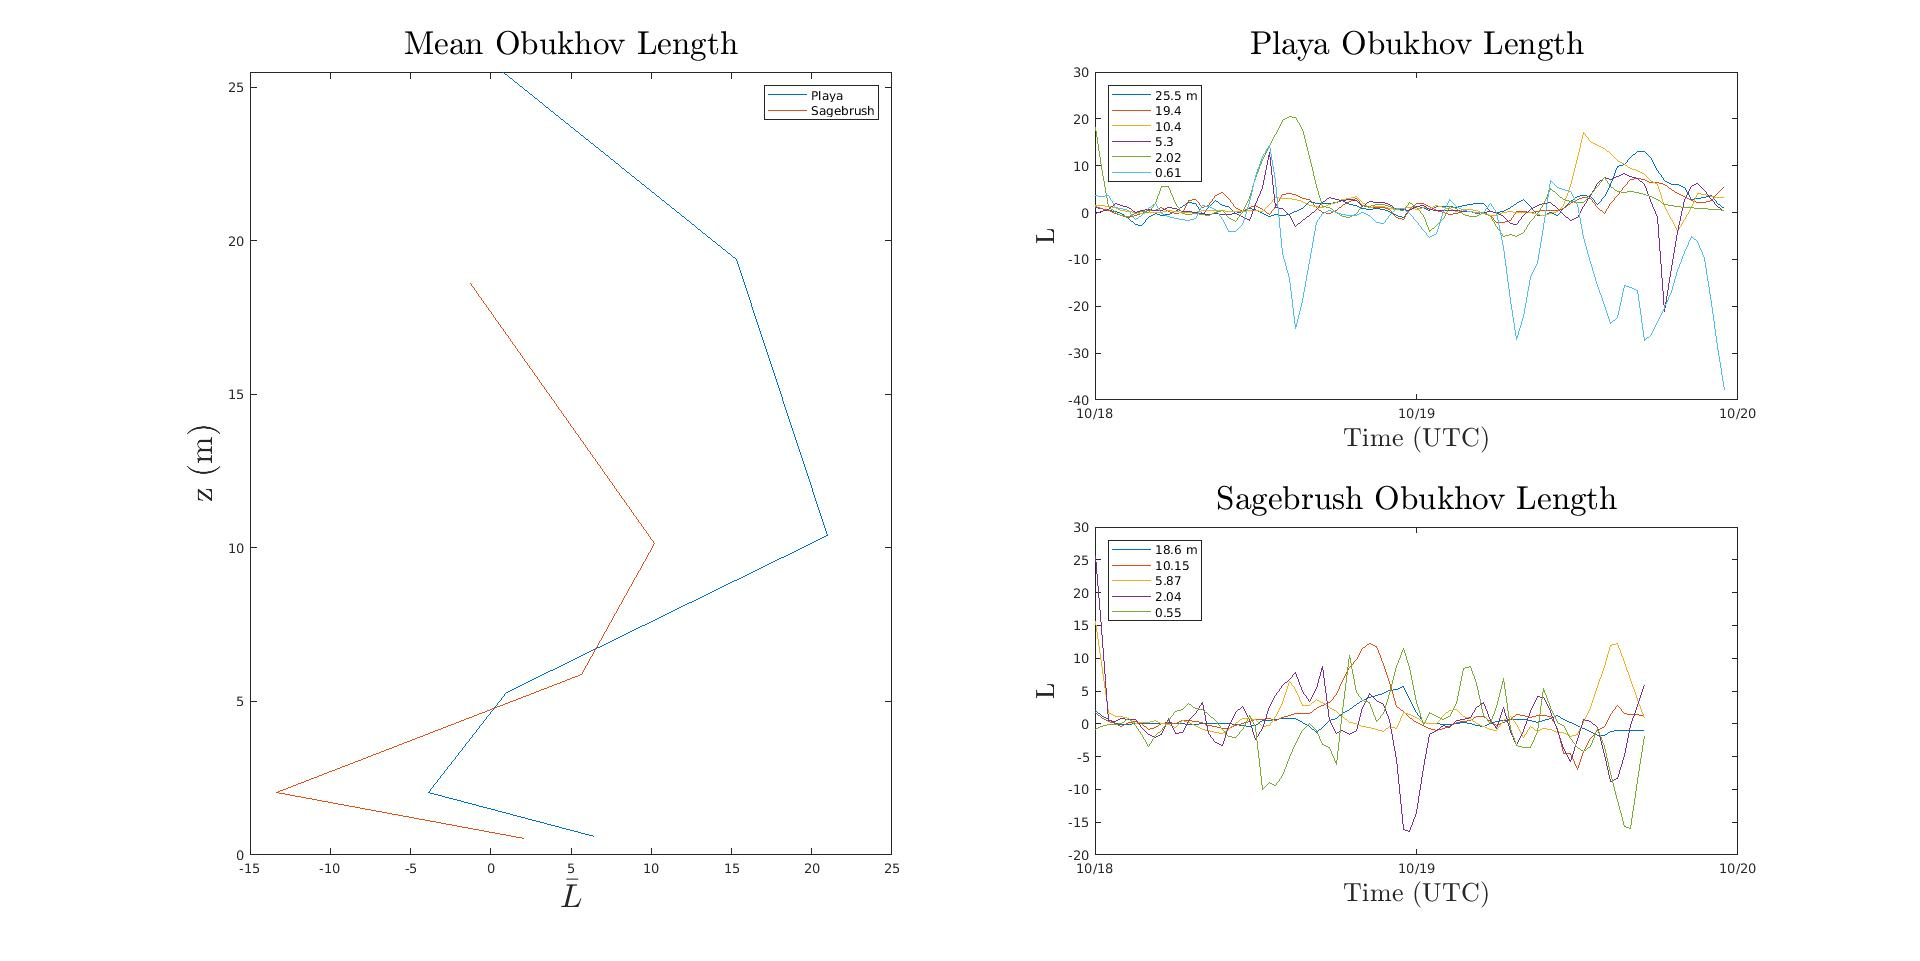
\includegraphics[width=\textwidth]{oblength}
	\caption{Obukhov length comparison. Mean Obukhov length plotted at each height (\textbf{left}), and time series (\textbf{right}) for both sites. Time series data were smoothed, giving little weight to outliers, using a variation of Loess Smoothing.}
	\label{fig:L}
\end{figure}



%Part 2 and 3~ Travis
To better understand the impacts of vegetation on boundary layer flow, examination of a highly convective time, 1500-1530 MST (2100-2130 UCT), was further analyzed. 
%Characteristics of this period include a mean wind speed and direction of.
 
The Probability Distribution Function (PDF) for this time period was calculated for each velocity component and temperature at all heights (Figure \ref{fig:pdf}). The largest contrast between the two sites exists in the PDF between the mean wind velocity component ($u$) and the temperature. Beginning with $u$ at the sagebrush site the velocity distribution's mean value shifts towards larger values with height, while at the Playa a more uniformed mean velocity is maintained across all heights. Additionally, insightful differences between the temperature PDF's between the two sites is observed. At the Sagebrush site, the 0.55 m and 2.04 m sonics report much larger mean temperature values ($\sim$19.5$^\circ$ C) than the other heights ($\sim$16.5$^\circ$ C) , while at the Playa site, the temperature remains uniform with height ($\sim$ 15-16.5 $^\circ$ C). Note at the Sagebrush site the temperature PDF at 0.55 m shows the largest variance. A potential explaination of this observation is that at the low near surface velocities due to the vegetation at Sagebrush decrease convection, hence increasing energy storage within this near surface layer, resulting in higher near-surface temperatures.  
%plot PDFs
\begin{figure}
	\centering
	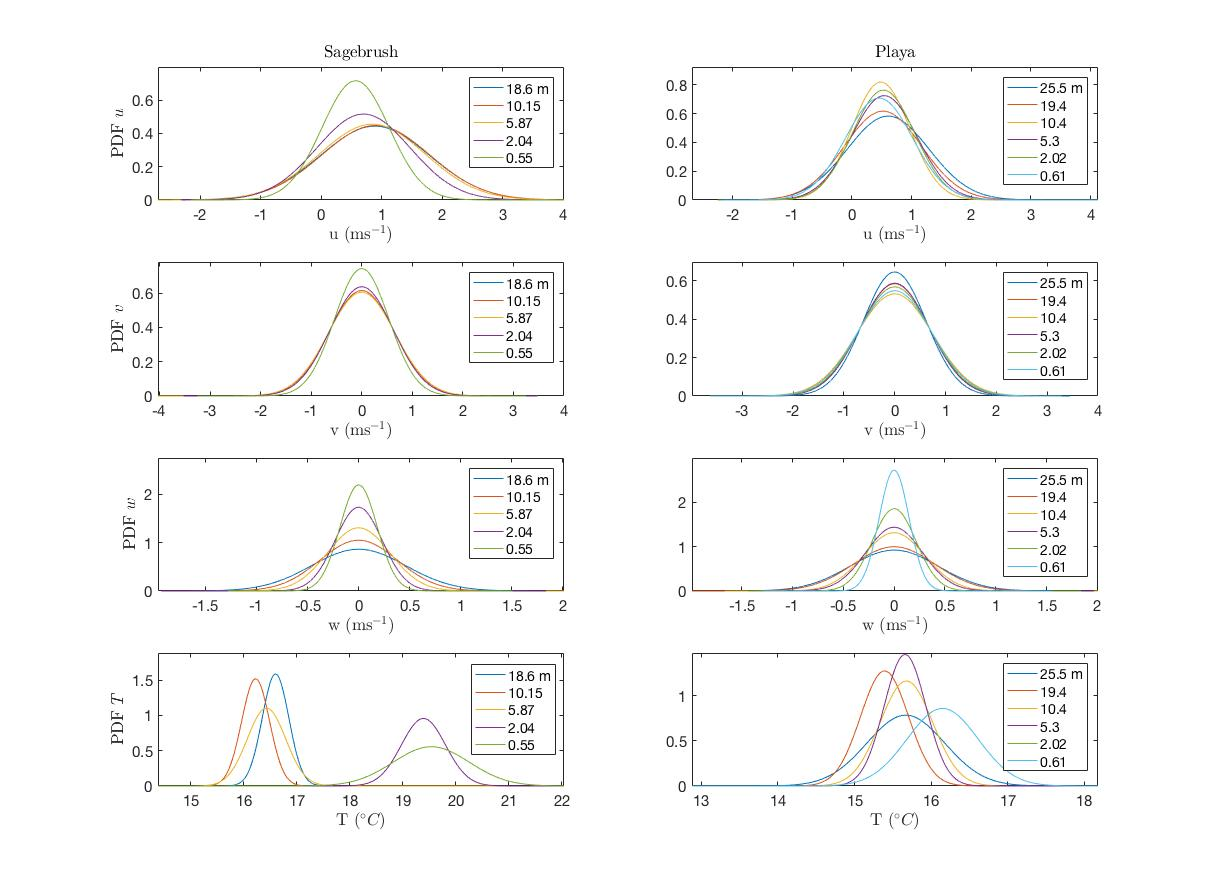
\includegraphics[width=\textwidth]{pdf}
	\caption{Collection of probability distributions from the Sagebrush (\textbf{left}) and the Playa (\textbf{right} sites). From top to bottom PDF $u$, PDF $v$,  PDF $w$ and PDF $T$ . }
	\label{fig:pdf}
\end{figure}
Table \ref{tab:kurt_sage} and Table \ref{tab:kurt_playa} present the kurtosis and skewness with height of velocity and temperature. The red and blue color boxes correlate to the near surface $u$ velocity at both sites. At the Sagebrush the skewness nears 0 at the surface, increasing with height. While the kurtosis remains less than 3. At the Playa, there is a positive skew near the surface on the mean wind direction, which decreases with height. A decreasing kurtosis in the same signal at the Playa is also observed.
%Create table of Skewness and Kurtosis
\begin{table}
\begin{tabular}{ |p{1cm}|p{2cm}|p{1cm}|p{1cm}|p{1cm}| p{1.5cm}|}

		\hline
		\multicolumn{6}{|c|}{Sagebrush} \\
		\hline\hline
		z (m) & Statistic & u &  v & w & T\\
		\hline
		18.6 & Kurtosis & 2.3731 & 3.1820 & 3.6346&  1.6588\\
		&Skewness & 0.3067 & 0.2446 & 0.8532 & -0.3490\\
		\hline
		10.15 & Kurtosis & 2.4933 & 3.4515 & 2.8027 &1.8469 \\
		&Skewness & 0.1651 & 0.1227 & 0.3879& -0.5126\\
        \hline
       	5.87 & Kurtosis & 2.6679 & 3.2820 & 3.8053 &2.0491 \\
       	&Skewness & 0.2694 & 0.1717 & 0.5359 & -0.6396\\
       	\hline
   		2.04 & Kurtosis & \cellcolor{red!25} 2.6868 & 3.6466  & 3.3045 & 2.0662  \\
   		&Skewness & \cellcolor{blue!25} 0.1876 & 0.3174 & 0.4101& -0.4458\\
   		\hline
		0.55 & Kurtosis & \cellcolor{red!25} 2.6739 & 3.1869 & 3.8168  & 2.4663\\
		&Skewness &\cellcolor{blue!25} 0.0655 & 0.3693 & 0.3859&0.7037\\
		\hline
		
\end{tabular}
\label{tab:kurt_sage}
\caption{Skewness and kurtosis values for the Sagebrush site on October 19th from 1500-1530 MST. }
\end{table}

\begin{table}
\begin{tabular}{ |p{1cm}|p{1.5cm}|p{1cm}|p{1.25cm}|p{1cm}| p{1.25cm}|}
	\hline
	\multicolumn{6}{|c|}{Playa} \\
	\hline\hline
	z (m) & Statistic & u &  v & w & T\\
	\hline
	25.5 & Kurtosis & 2.1075 & 2.5910 & 3.5269 &  2.2656\\
	&Skewness & 0.1212 & -0.2004 & 0.7672 & 0.5295\\
	\hline
	19.4 & Kurtosis & 2.2519 & 2.8332 & 3.4123 &1.6080 \\
	&Skewness & 0.2287 & -0.2862 & 0.7324 & 0.1421\\
	\hline
	10.4 & Kurtosis & 2.8320 & 1.9469 & 3.0079 &4.6 \\
	&Skewness & 0.3884 & 0.1464 & 0.3786 &1.2276\\
	\hline
	5.3 & Kurtosis & 2.9033 & 2.1528  & 3.1285 & 3.2123  \\
	&Skewness & 0.1862 & 0.1298 & 0.4560 & 0.9190\\
	\hline
	2.02 & Kurtosis &\cellcolor{red!25} 3.0038 & 2.0993 & 3.2620  & 2.3460\\
	&Skewness & \cellcolor{blue!25} 0.3980 & -0.0969 & 0.4160 & 0.6531\\
	\hline
	0.61 & Kurtosis & \cellcolor{red!25} 3.1414 & 1.9599 & 3.3634  & 2.3473\\
	&Skewness & \cellcolor{blue!25} 0.5253 & -0.1403 & 0.2770 &0.6531\\
	\hline
\end{tabular}
\label{tab:kurt_playa}
\caption{Skewness and kurtosis values for the Playa site on October 19th from 1500-1530 MST. }
\end{table}
Figure \ref{fig:cdf} presents the Cumulative Distribution Function (CDF). Focusing on the third row (CDF $w$) one can now see of the increased distribution of vertical velocities with height at both sites. This is due to the convective nature of the period of interest. Figure \ref{fig:autocorr} presents the autocorrelation function for the velocity components and the temperature at both sites. The autocorrelation was computed for the 30 minutes of interest, 15 minutes is presented. $u$, $v$, and $T$ show fairly linearly decays with time, while $w$ decays rapidly to 0. Interesting features in Figure \ref{fig:autocorr} are seen in the autocorrelation of $u$ at the Sagebrush and Playa. At the Sagebrush we observe a more rapid decay of correlation at the lower heights, while at the Playa, all heights share the same correlation with time (decreasing at similar rates). 
%plot CDFs
\begin{figure}
\centering
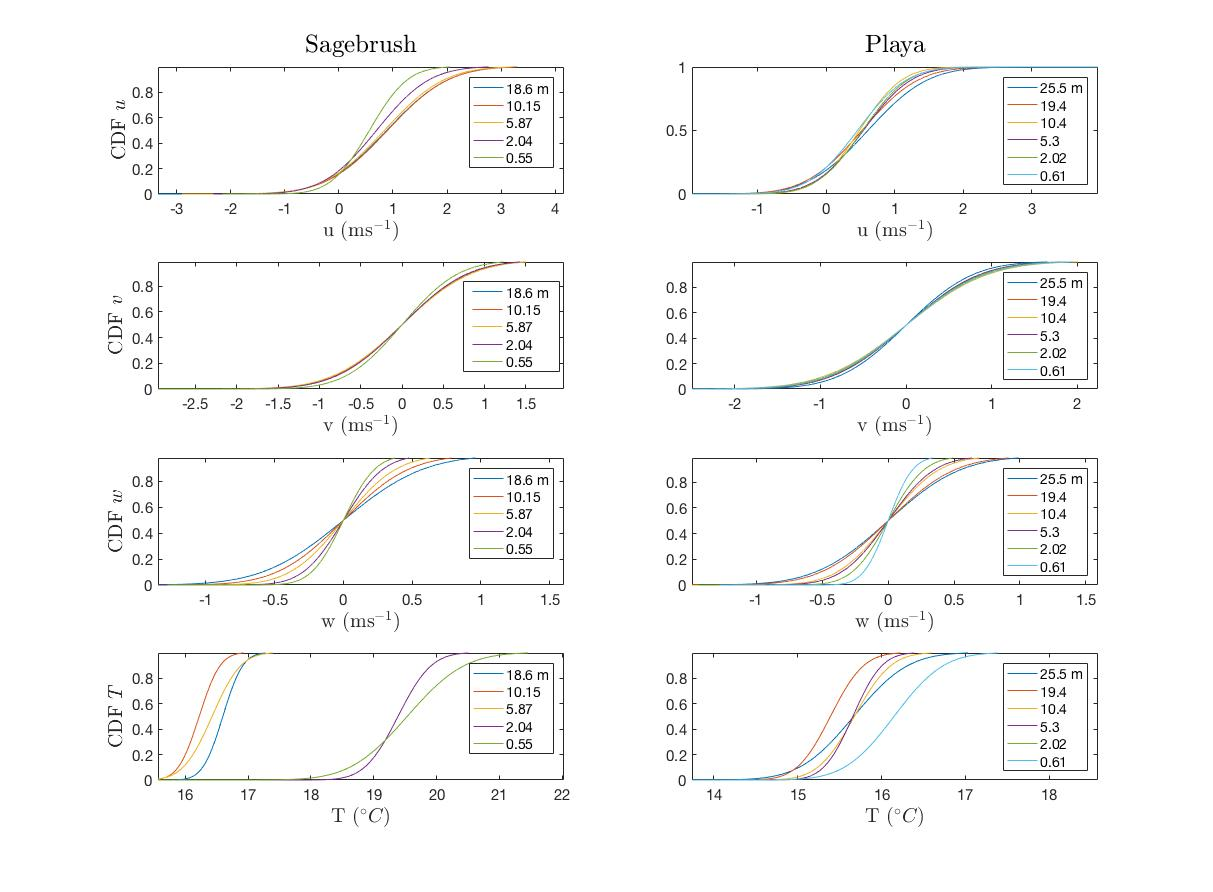
\includegraphics[width=\textwidth]{cdf}
	\caption{Collection of cumulative distributions from the Sagebrush (\textbf{left}) and the Playa (\textbf{right} sites). From top to bottom CDF $u$, CDF $v$,  CDF $w$ and CDF $T$ . }
\label{fig:cdf}
\end{figure}
%plot Autocorr
\begin{figure}
	\centering
	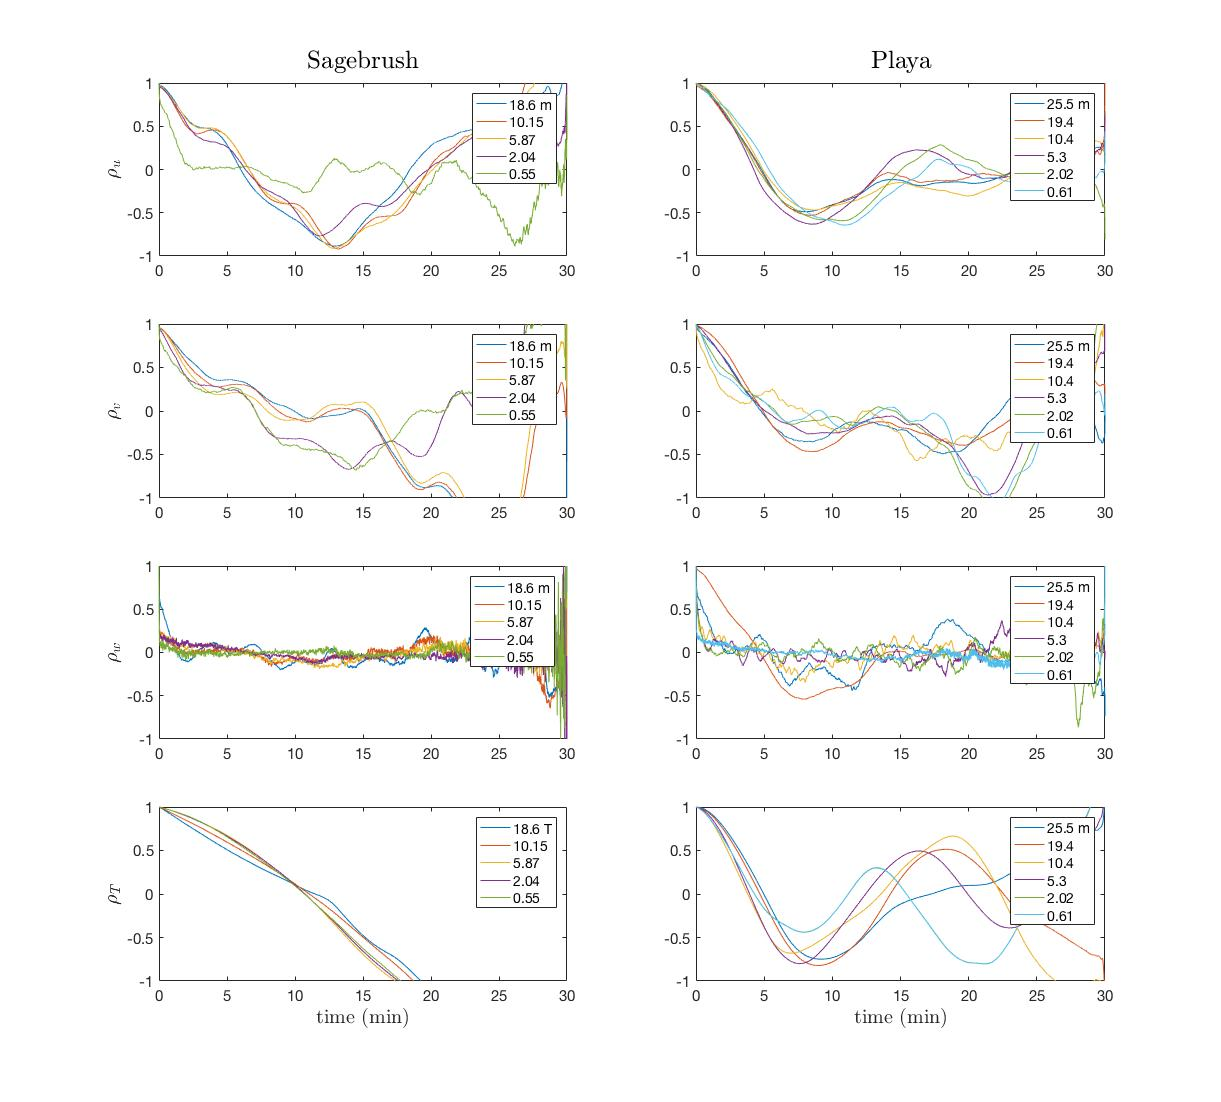
\includegraphics[width=\textwidth]{auto_corr_fig}
	\caption{Collection of autocorrelations from the Sagebrush (\textbf{left}) and the Playa (\textbf{right} sites). From top to bottom $\rho$ $u$, $\rho$ $v$,  $\rho$ $w$ and $\rho$ $T$ . }
	\label{fig:autocorr}
\end{figure}
Additionally, further turbulence analysis was performed on the data from the two sites. Figure \ref{fig:u_T} presents the temperature with height (right) of the two sites, while the left column presents (from top to bottom) the mean velocity with height, instantaneous plots of $u^\prime$,  $v^\prime$, and $w^\prime$ with height. The data presented is only of the period of interest. From the temperature profile, we observe a large energy storage (2$^\circ$C) at the surface layer compared to the Playa. In the mean velocity profile the impact of the sagebrush on the mean flow, creating a large drag at the surface, is clearly observed. Examination of the fluctuations reveals the fluctuations in the mean wind direction are larger in magnitude at the Playa with less variance compared to the Sagebrush, while the converse is observed for the cross wind component. The vertical fluctuations at both sites appear to increase in variance and magnitude with height.  
%plot u mean, T mean u' v' and w'
\begin{figure}
	\centering
	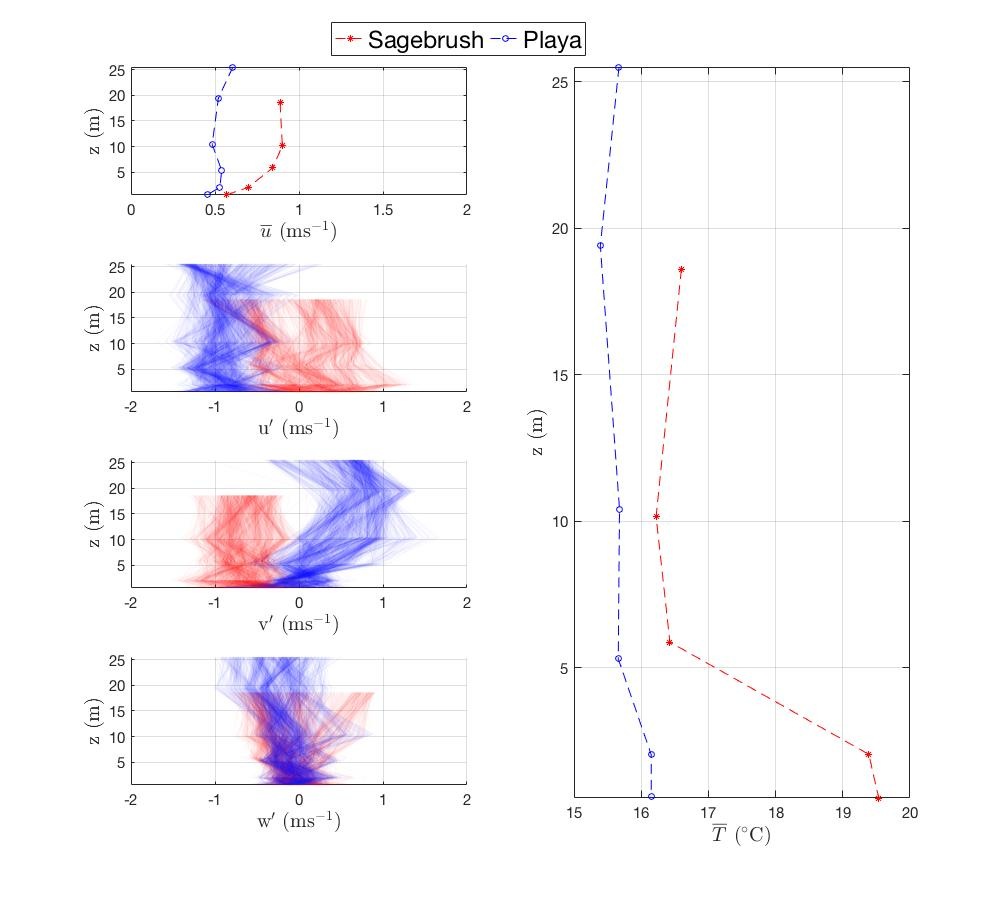
\includegraphics[width=\textwidth]{u_T}
	\caption{Sagebrush (red) and Playa (blue) mean velocity (top left), instantaneous velocity fluctuations at 20 Hz (left) and temperature (right) for each height during period of interest, 1500-1530 MST on October 19th, 2012}
	\label{fig:u_T}
\end{figure}
Figure \ref{fig:mom_05} and Figure \ref{fig:mom_20} presents the fluctuation correlations between the velocity components and their respective kinematic heat fluxes (Figure \ref{fig:mom_05} at 0.5 m and Figure \ref{fig:mom_20} at 20 m). At both heights for the velocity correlations the Sagebrush appears to contain larger fluctuations in each variable (larger spread). Suggesting an increase in TKE at this site. As expected at 0.5 m the heat flux correlations have very small velocity fluctuations, however larger temperature fluctuations exist, suggesting the surface heterogeneity influencing the flow. Larger temperature fluctuations are seen at the Sagebrush then the Playa at the 0.5 m, suggesting the impact of temperature heterogeneity is affecting the flow more so at the Sagebrush site than the Playa site. Examination of the 20 m heat flux correlation suggests that the temperature fluctuations at both site match fairly well in magnitude, thus concluding the effect observed at the lower height from the Sagebrush, has been washed out by 20 m. 
%correlation plots
\begin{figure}
	\centering
	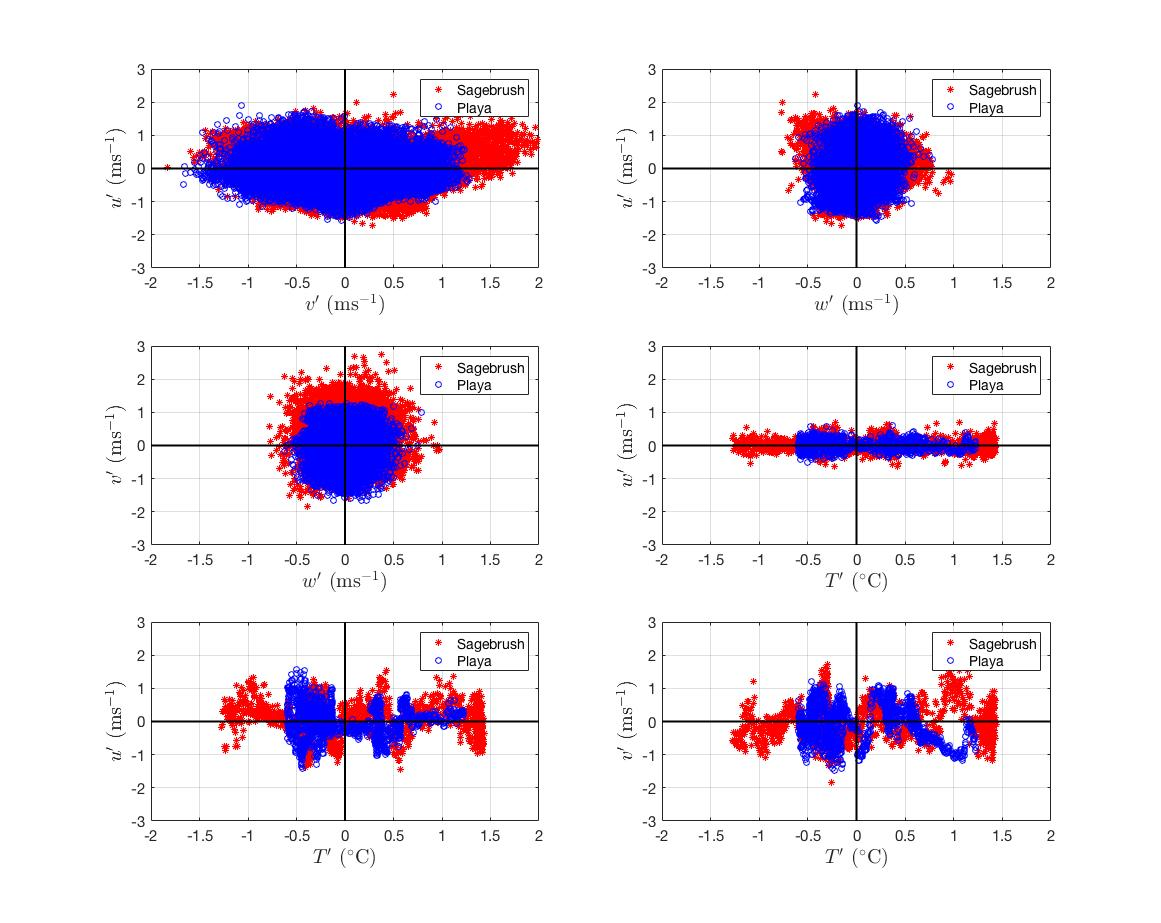
\includegraphics[width=\textwidth]{momentum_corr_05m}
		\caption{Correlations for momentum and heat flux for 0.5 m during period of interest, 1500-1530 MST on October 19th, 2012}
	\label{fig:mom_05}
\end{figure}
\begin{figure}
	\centering
	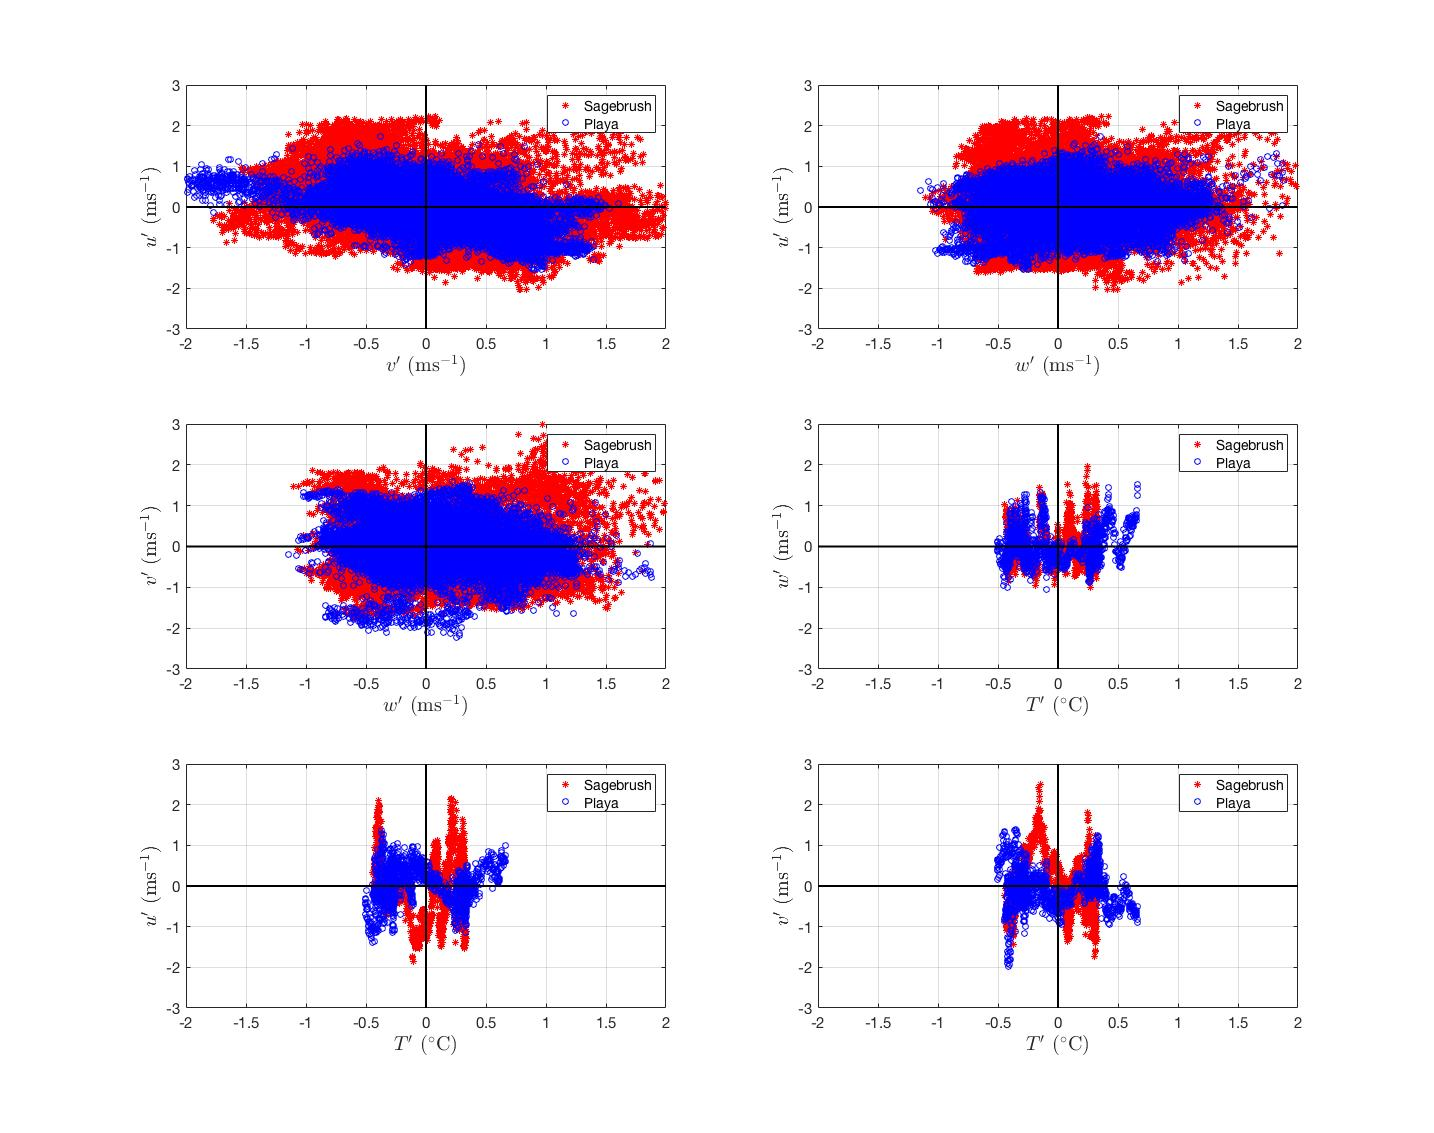
\includegraphics[width=\textwidth]{momentum_corr_20m}
		\caption{Correlations for momentum and heat flux for 20 m during period of interest, 1500-1530 MST on October 19th, 2012}
	\label{fig:mom_20}
\end{figure}


%Matt talks about part 4 and 5
\subsection{Dissipation}
Taylor's Frozen hypothesis is utilized to determine the dissipatin rate and Kolmogorv length of the turbulent eddies. Taylor hypothesized in 1938 that for special cases turbulence "may be considered "frozen" as it advects past a sensor."\cite{Stull} This allows for turbulent scales to be determined by a time analysis of the mean velocity. If the mean velocity is much greater than the turbulent scales, Taylor put forth that " and eddy of diameter &\lambda$ is advected at mean wind speed M, then the time period P for it to pass by a stationary sensor is given by P = $\lambda$/M."\cite{Stull} If an eddy does not change in time as it is advected past the sensor then some variable, ie. temperature, velocity, etc. on the leading edge of the edyy vs the same variable on the trailing edge of the eddy can be considered frozen, and thus the time and spatial components of variation in the variable may be correlated as $\frac{\partial \zeta}{\partial x_D}$ where x_D is parallel to the mean wind. Taylor's hypothesis holds when $\frac{d\zeta}{dt} = 0$. Using the definition of total derivative this yields
\begin{equation} \label{eq:taylor}
\frac{\partial \zeta}{\partial t} = -U\frac{\partial \zeta}{\partial x} - V\frac{\partial \zeta}{\partial y} - W\frac{\partial \zeta}{\partial z}
\end{equation}

Utilizing Taylor's Hypothesis the Dissipation Rate (m^2/s^3is calculated using 
\begin{equation} \label{eq:diss}
\epsilon (\zeta ,t) = 2\nu \int_{\zeta}^{\infty} \zeta '^2E(\zeta ',t)d\zeta 
\end{equation}
and the Kolmogorov length (mm)is calculated as 
\begin{equation} \label{eq:kolm_length}
\frac{\nu^3}{\epsilon}^{1/4}*10^3
\end{equation}

The dissipation rate and Kolmogorov length were calculated over several 30 minute time periods and compared for the Playa and Sagebrush sites at the 10 m height and are presented in table \ref{tbl:diss}. 
\begin{table}[h] \label{tbl:diss}
\captionof{table}{Dissipation Rate and Kolmogorov Length}
\begin{minipage}[b]{0.45\linewidth}
\centering
\begin{tabular}{|c||c|c|}
	\hline
	\multicolumn{3}{|c|}{Dissipation Rate} \\
	\hline
	& Playa & Sagebrush \\
	\hline
	6:00 am & 0.0019 & 0.00035 \\
	6:30 am & 0.0021 & 0.0011 \\
	7:00 am & 0.00077 & 0.00055 \\
	\hline
\end{tabular}
\end{minipage}%
\begin{minipage}[b]{0.45\linewidth}
\centering
\begin{tabular}{|c||c|c|}
	\hline
	\multicolumn{3}{|c|}{Kolmogorov Length} \\
	\hline
	& Playa & Sagebrush \\
	\hline
	6:00 am & 1.55 mm & 2.36 \\
	6:30 am & 1.51 & 1.79 \\
	7:00 am & 1.93 & 2.11 \\
	\hline
\end{tabular}
\end{minipage}%
\end{table}
It can be seen that the dissipation rates and Kolmogorov lengths are similar for both sites. When the same quantities are calculated at the 2 m height however the results begin to vary wildly. While the Playa sites have nearly identical values the dissipation rate for the Sagebrush goes to nearly 800 and the Kolmogorov length goes to 0.006 mm. This indicates that vegetation in the Sagebrush site has enough surface roughness to increase the viscous sublayer substantially. 

\subsection{Turbulence Spectra}
Turbulence Spectra is a tool we use to analyze the energy density at various frequencies. Turbulence can be considered to be composed of various sized eddies which transfer energy in the TKE from larger sized eddies to smaller. Richardson proposed that eddies are unstable and as they break down they "cascade" thier energy to the smaller scales. The smallest ediies eventually disspiate the kinetic energy through viscous forces as there is no coherent scale for eddies to exist at the highest wavenumbers.\cite{Pope} The energy spectra of the variable in question can be broken down into three ranges. An energy producing range, an inertial subrange and a dissipation range. 

The turbulence spectra was calculated for each coordinate direction of wind as well as temperature. Figures \ref{fig:S_uu10m} through \ref{fig:S_tt10m} show each spectra for the associated variable.
\begin{figure}[h]
	\centering
	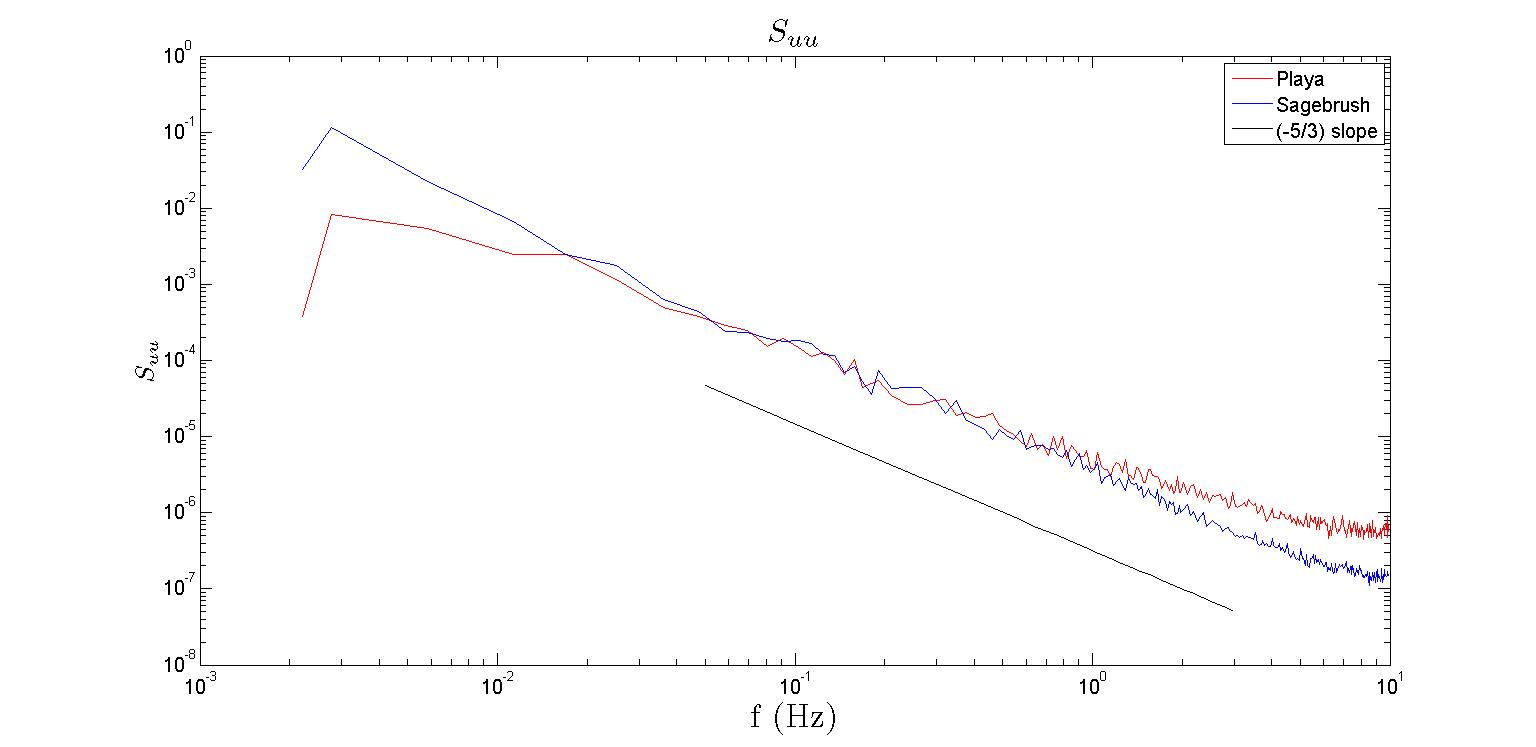
\includegraphics[width=\textwidth]{S_uu10m.jpg}
	\caption{Turbulence spectra for uu}
	\label{fig:S_uu10m}
\end{figure}
\begin{figure}[h]
	\centering
	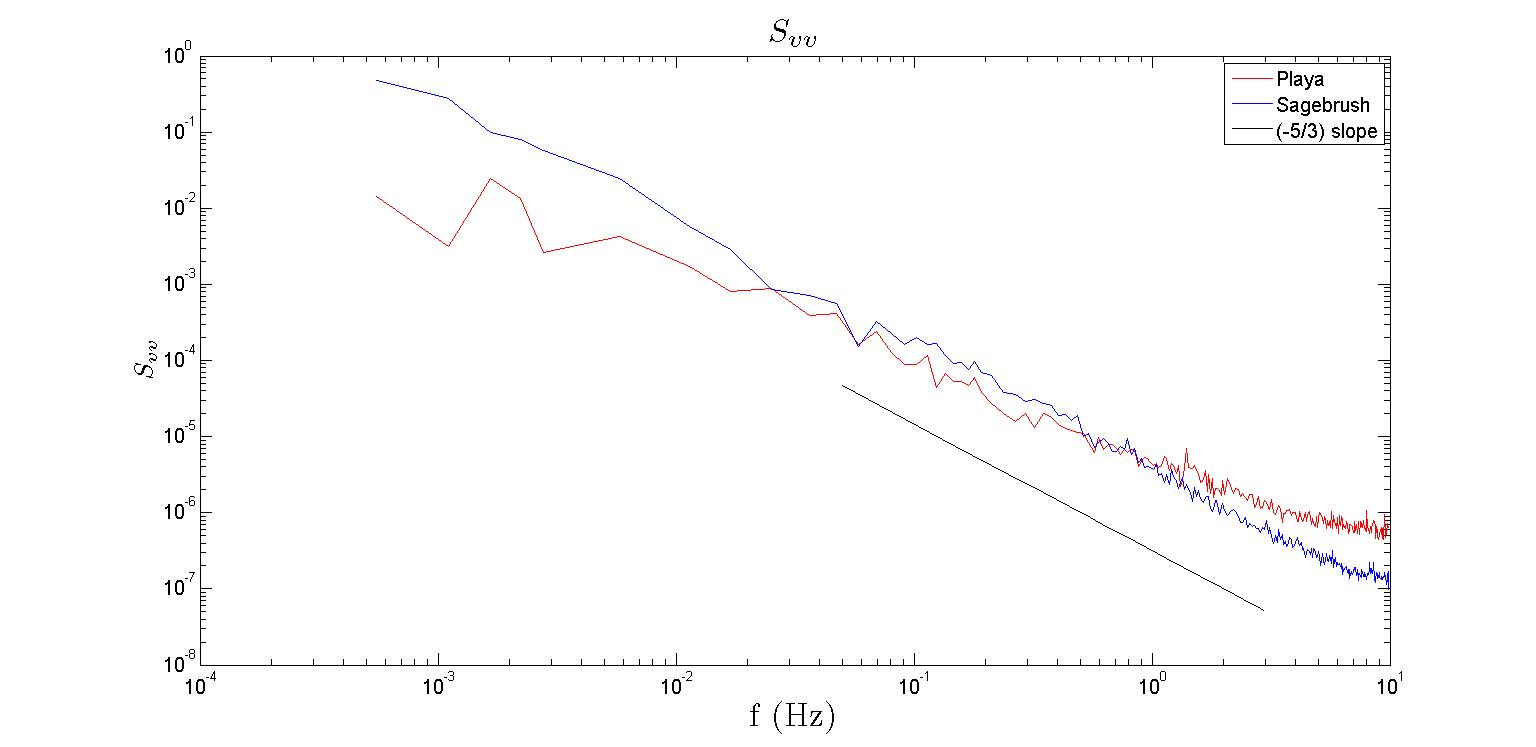
\includegraphics[width=\textwidth]{S_vv10m.jpg}
	\caption{Turbulence spectra for vv}
	\label{fig:S_vv10m}
\end{figure}
\begin{figure}[h]
	\centering
	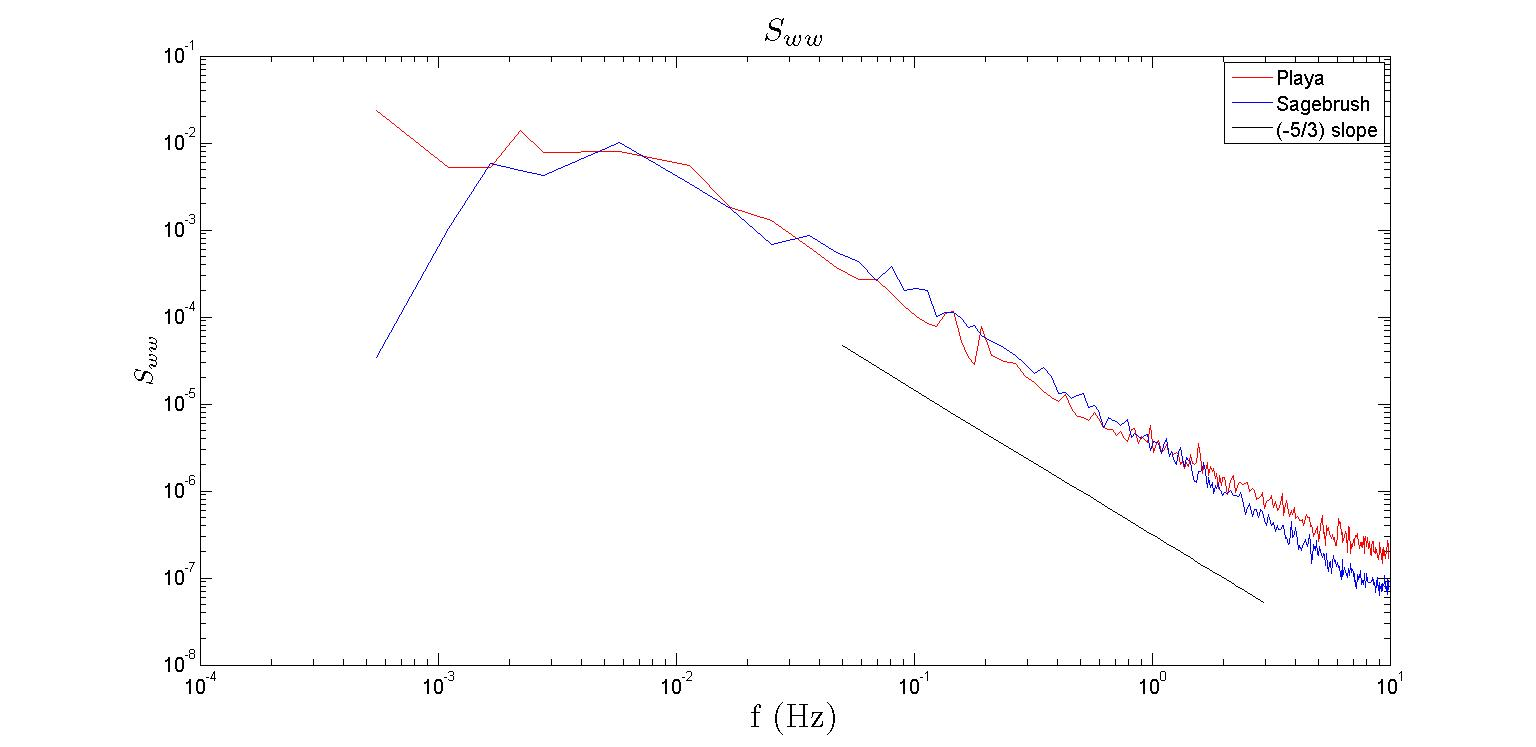
\includegraphics[width=\textwidth]{S_ww10m.jpg}
	\caption{Turbulence spectra for ww}
	\label{fig:S_ww10m}
\end{figure}
\begin{figure}[h]
	\centering
	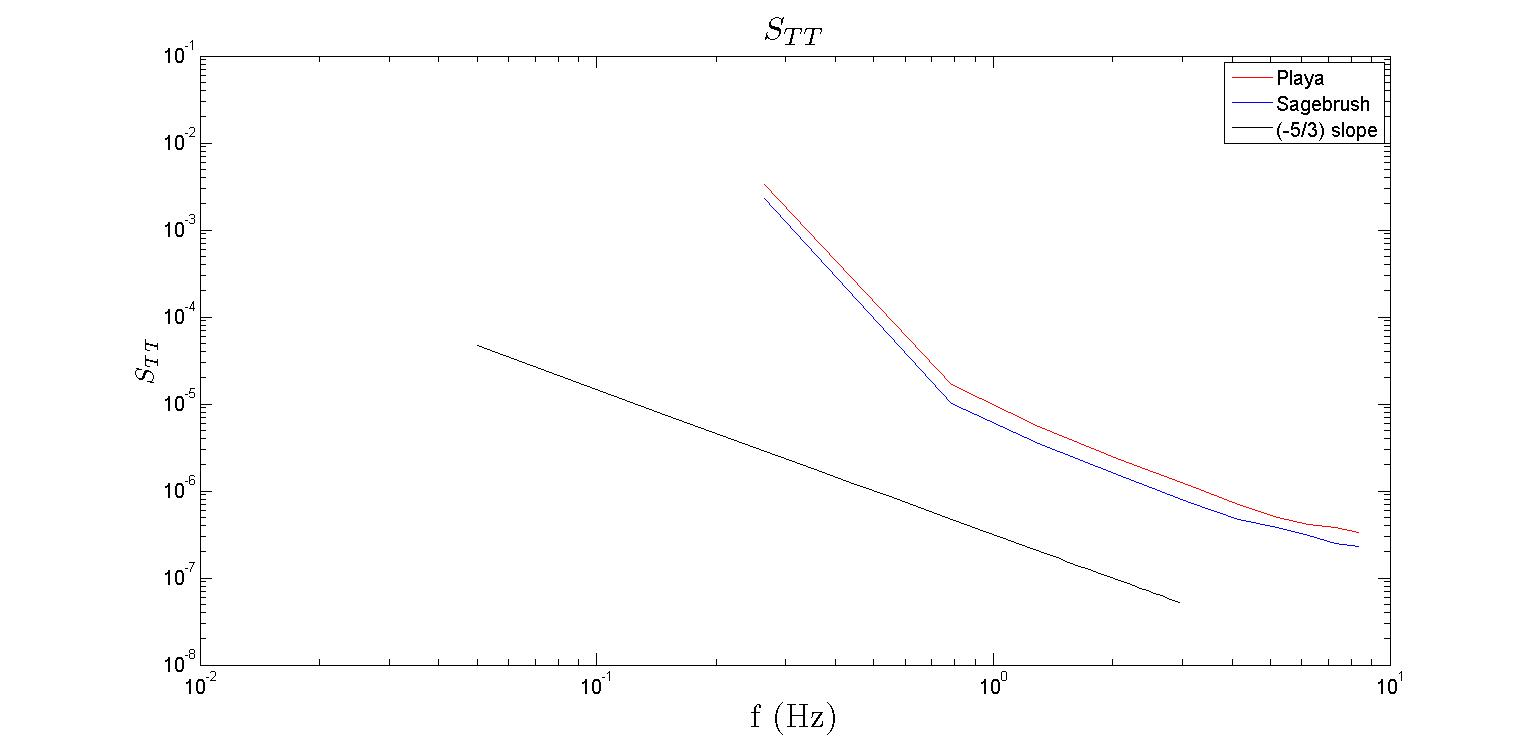
\includegraphics[width=\textwidth]{S_tt10m.jpg}
	\caption{Turbulence spectra for tt}
	\label{fig:S_tt10m}
\end{figure}

For each variable at the 10 m height we see that the Sagebrush site has a larger production range. Both the Sagebrush and Playa sites also follow the classical -5/3 power law in the inertial subrange. For convienence the 5/3 line is plotted as a reference. The Sagebrush site has a steeper slope at higher frequencies. This tells us that the dissipation is higher for Sagebrush. This is expected as it also has higher production, and increased production must lead to increased dissipation in order to conserve energy.

The turbulence spectra was also calculated at the different heights of the tower. At the 2 m height we see that the Playa site has very similar characteristics.  However the Sagebrush site does not follow the trend we expect at all. There are no distinct regions in the turbulence spectra for production / dissipation and we see no energy cascade. Figure \ref{fig:S_uu} shows the spectra plotted for uu.
\begin{figure}[h]
	\centering
	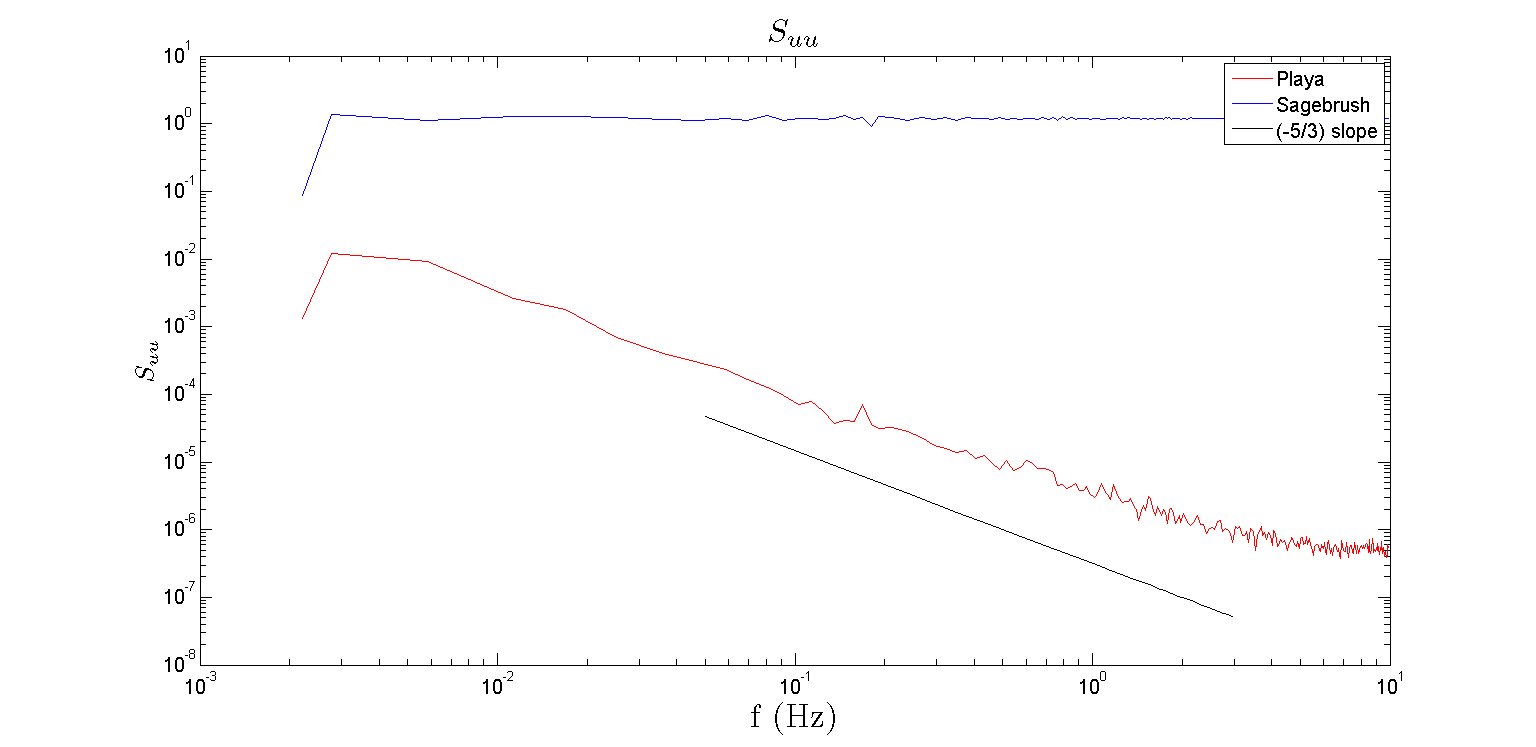
\includegraphics[width=\textwidth]{S_uu.png}
	\caption{Turbulence spectra for uu at 2 m height}
	\label{fig:S_uu}
\end{figure}
At the 2 m height the vegetation at Sagebrush causes enough surface roughness that the assumptions we use for Taylor's hypothesis and the Kolmogorov energy cascade do not hold; namely that z << z_0 is not true. 

The cospectra for the variables of interest are also plotted (figures \ref{fig:S_uw10m} through \ref{fig:S_vw}) and show the same trends as the spectra. This is expected as Kolmogorov's hypothesis holds that at smal scales turbulence may be considered isotropic.\cite{Pope}
\begin{figure}[h]
	\centering
	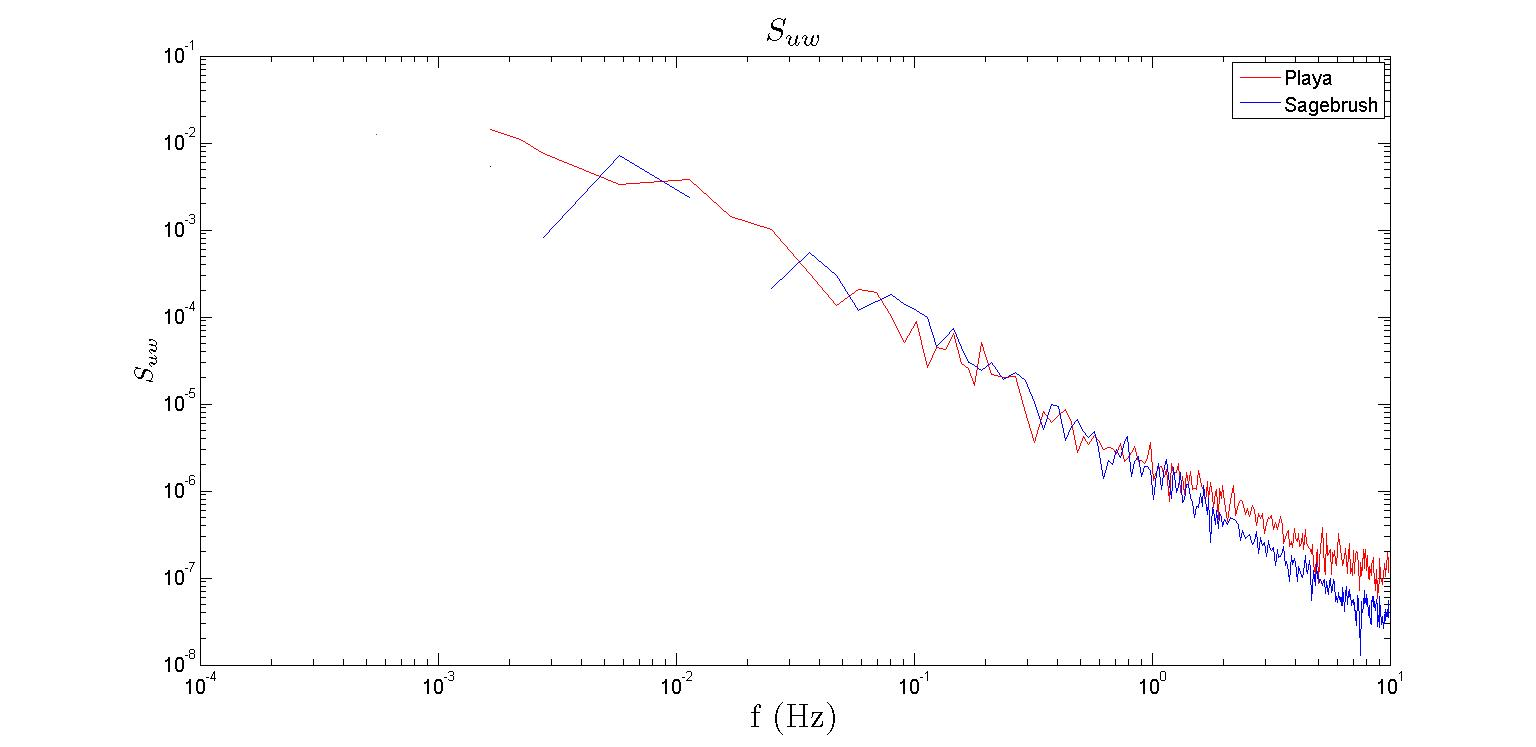
\includegraphics[width=\textwidth]{S_uw10m.jpg}
	\caption{Turbulence spectra for uw}
	\label{fig:S_uw10m}
\end{figure}
\begin{figure}[h]
	\centering
	\includegraphics[width=\textwidth]{S_vw10m.jpg}
	\caption{Turbulence spectra for vw}
	\label{fig:S_vw10m}
\end{figure}

\section{Conclusion}
 %main conclusions
 In an effort the better understand the impact of the surface roughness heterogeneities between the Playa and Sagebrush sites the authors have confined their findings to the following key results. 
 \begin{itemize}
 	\item
 	The Sagebrush site has increased dissipation, energy storage, and larger contribution of high frequency eddies as a result of the increased surface roughness.
 	\item
 	The Playa site demonstrated stronger autocorrelations along all heights.
 	\item 
 	The impacts of the vegetation at the Sagebrush site diminish by 10 m.
 \end{itemize}
 
 
 %Additional work
 Additionally the authors would like to examine the impact of different de-trending times, such as \cite{} whose analysis utilizes a 5 minute de-trending period for evening transitions. Furthermore a more in depth analysis utilizing Multi-Resolution Decomposition during the time period  to derive a time and length scale associated with the surface roughness heterogeneity. 

\newpage
\bibliographystyle{apalike}
\bibliography{references}
\end{document}
